
\chapter{Methods}




\section{Neuron and network model}

This section will go into detail about the computations behind the network which was developed by
\cite{sacramento2018dendritic} and expanded by \cite{Haider2021}.


\subsection{Network architecture}

\begin{figure}
  \centering
  \begin{minipage}{0.5\textwidth}
    \centering
    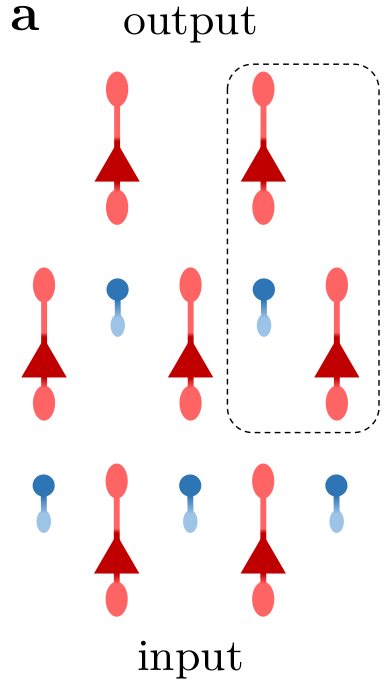
\includegraphics[width=0.9\textwidth]{network_a}
  \end{minipage}\hfill
  \begin{minipage}{0.4\textwidth}
    \centering
    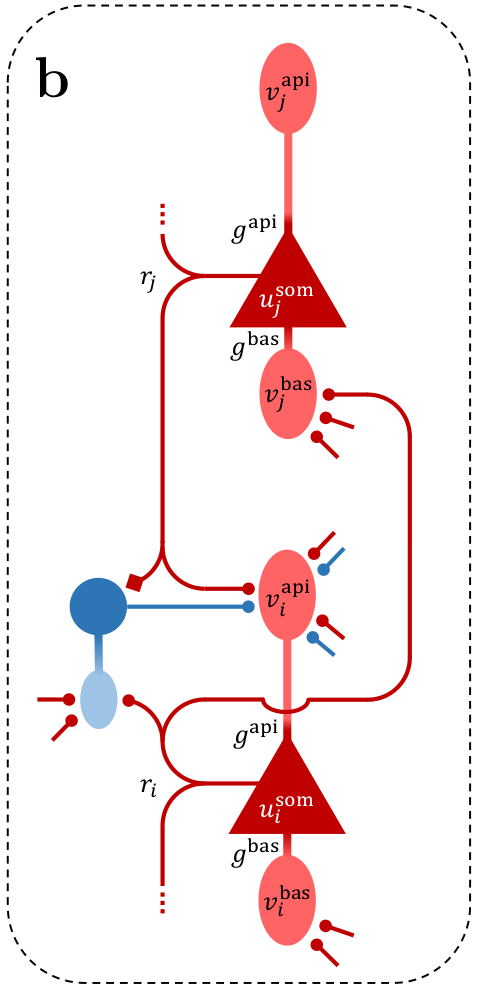
\includegraphics[width=0.9\textwidth]{network_b}
  \end{minipage}
  \caption{Network structure, from \cite{Haider2021}. \textbf{a:} pyramidal- (red) and interneurons (blue) in a network
    of three layers. Note the fact that the number interneurons in a layer is equal to the number of pyramidal neurons
    in the subsequent layer\protect\footnotemark. \textbf{b:} connectivity within the highlighted section. Feedback
    pyramidal-to-interneuron connections (displayed with rectangular synapse) transmit pyramidal somatic potential
    directly and connect to a single interneuron. This enables these interneurons to learn to match their corresponding
    next-layer pyramidal neurons. All other synapses (circles) transmit the neuron somatic activation $\phi (u^{som})$
    and fully connect their origin and target populations.}
  \label{fig-network}
\end{figure}

\footnotetext{{Note that the input layer is displayed as having interneurons here. This appears to be a mistake in the
      graphic. In the implementation, interneurons are only modelled in hidden layers.}}

The model which was original described by \cite{sacramento2018dendritic} contains a strongly recurrent network
structure, which will be explained in this section. It can be functionally separated into layers, with information
flowing from the input layer through one or more hidden layers to the output layer. Neurons at the input layer receive
no feedback connections and serve primarily to apply a low-pass filter over the input sequence injected into their
membrane. Output layers have no interneurons, and are usually modeled as pyramidal neurons without an apical
compartment. Hidden layers consist of a pyramidal- and an interneuron population, which are fully connected to each
other in both directions (see Figure \ref{fig-network}). Feedforward connections between layers are facilitated by
all-to-all connections between their respective pyramidal neurons and innervate the basal compartments. Feedback
connections from superficial layers and interneurons on the other hand arrive at apical compartments. Interneurons
receive lateral input from all pyramidal neurons of their layer, as well as feedback information from superficial
pyramidal neurons. These feedback connections are special, since they connect one pyramidal neuron to exactly one
interneuron. Instead of transmitting neuronal activation, this connection relays somatic voltage directly. The resulting
dynamics share features of electrical synapses, which will be discussed in Section \ref{sec-electric-syns}. To
understand what purpose this connectivity serves in our model, neuron and plasticity models require some elaboration.


\subsection{Neuron models}\label{sec-neurons}



The network contains two types of multi-compartment neurons; Pyramidal neurons with three compartments each, and
interneurons with two compartments each. They integrate synaptic inputs into dendritic potentials, which leak into the
soma with specific conductances. Note that vector notation will be used throughout this section, and $u_l^P$ and $u_l^I$
denote the column vectors of pyramidal- and interneuron somatic voltages respectively. Synaptic weights $W$ are likewise
assumed matrices.The activation $r_l^P$ of pyramidal neurons at layer $l$ is given by applying the synaptic transfer
function $\phi$ to to their somatic potentials $u_l^P$:
\begin{align}
  r_l^P   & = \phi(u_l^P)                                                        \\
  \phi(x) & = \begin{cases}
                0                                   & \textrm{if } \ x < -\epsilon \\
                \gamma \ log(1+e^{\beta(x-\theta)}) & \textrm{if } \ x < \epsilon  \\
                \gamma \ x                          & \textrm{otherwise}
              \end{cases}
\end{align}

where $\phi$ acts componentwise on $u$ and can be interpreted as a smoothed variant of ReLu \todo{cite} with scaling
factors $\gamma$, $\beta$, $\theta$ and threshold parameter $\epsilon$. The derivative somatic membrane potentials of
layer $l$ pyramidal neurons is given by:

\begin{align}
  C_m \dot{u}_l^P & = - g_l u_l^{som} + g^{bas} v_l^{bas} + g^{api} v_l^{api} \label{eq-pyr-dynamics-rate}
\end{align}

where $v_l^{bas}$ and $v_l^{api}$ are the membrane potentials of basal and apical dendrites respectively, and $g^{bas}$
and $g^{api}$ their corresponding coupling conductances. The membrane capacitance $C_m$ is $1$ in all relevant
simulations, and will be omitted from all Equations from here on out.


In the original model, dendritic compartments have no persistence between simulation steps. Thus, they are defined at
every timestep $t$ through incoming weight matrices and presynaptic activities:

\begin{align}
  v_l^{bas}(t) & = W_l^{up} \ \phi(u_{l-1}^P(t)) \label{eq-v-bas-rate}                                     \\
  v_l^{api}(t) & =  W_l^{pi} \ \phi(u_l^I(t)) \ + \  W_l^{down} \ \phi(u_{l+1}^P(t)) \label{eq-v-api-rate}
\end{align}

Weight nomenclature conforms to the python implementation of the network by \cite{Haider2021}; Weights are indexed by
the layer in which the target neuron is located and belong to one of four populations. Feedforward and feedback
pyramidal-to-pyramidal connections arriving at layer $l$ are denoted $W_l^{up}$ and $W_l^{down}$ respectively. Lateral
pyramidal-to-interneuron connections are denoted with $W_l^{ip}$ and their corresponding feedback connections with
$W_l^{pi}$. Since the input layer contains no synapses, indexing begins with $0$ for the first hidden layer. \newline

Interneurons integrate synaptic information by largely the same principle, but instead of feedback information arriving
at the apical compartment, it is integrated directly into the soma. Through this, interneurons functionally resemble the
original neuron from \cite{urbanczik2014learning} most closely.

\begin{align}
  C_m \dot{u}_l^I & = - g_l u_l^{I} + g^{dend} v_l^{dend} + i^{nudge, I}\label{eq-intn-dynamics} \\
  i^{nudge, I}    & = g^{nudge, I} u_{l+1}^P                                                     \\
  v_l^{dend}      & = W_l^{ip} \ \phi(u_{l}^P)
\end{align}

where $ g^{nudge, I}$ is the interneuron nudging conductance, and $u_{l+1}^P$ is the somatic voltage of a corresponding
pyramidal neuron in the next layer. Since each interneuron is innervated by exactly one pyramidal neuron and vice versa,
they will be called each others \textbf{sister neurons} from here on.\todo{discuss whether this 1 to 1 style connection
  is plausible!}. Pyramidal neurons in the output layer $N$ effectively behave like interneurons, as they receive no input
to their apical compartment. Instead, the target  activation $u^{tgt}$ is injected into their soma:

\begin{align}
  C_m \dot{u}_N^P & = - g_l u_N^{P} + g^{bas} v_N^{bas} + i^{nudge, tgt} \\
  i^{nudge, tgt}  & = g^{nudge, tgt} u^{tgt}
\end{align}


These neuron dynamics correspond closely to those by \cite{urbanczik2014learning}, including the extension to more than
two compartments which was proposed in the paper. It should be noted however, that they are simplified in some key ways.
Primarily, dendritic couplings and nudging are not relative to the somatic or some reversal potential (i.e. $i^{nudge,
      tgt}= g^{nudge, tgt} (u^{tgt} - u_N^P )$), but are simplified to absolute values. \todo{Figure out if this makes a
  difference. maybe create a second branch to try them out? }








\section{Urbanczik-Senn Plasticity}\label{sec-urb-senn-plast}

The synapses in the network are all modulated according to variations of the "Urbanczik-Senn" plasticity rule
\citep{urbanczik2014learning}, which will be discussed in this section. \todo{add paragraph about relevance of
  urbanczik-senn}

The plasticity rule requires the postsynaptic neuron to have one somatic and at least one dendritic compartment, to the
latter of which synapses connect. The membrane potential of the dendritic compartment leaks into the somatic compartment
as described in Equation \ref{eq-intn-dynamics}.


Functionally, the plasticity rule changes the synaptic weight in such a way, as to minimize discrepancies between
somatic and dendritic potential. The change in weight for a synapse fron neuron $j$ to neuron $i$ is thus given by:

\begin{align}
  \dot{w}_{ij}    & = \eta \ ( \phi(u_i^{som}) - \phi(\hat{v}_i^{bas}) ) \ \phi(u_j^{som})^T \\
  \hat{v}_i^{bas} & = \alpha \  v_i^{bas}
\end{align}

with learning rate $\eta$ and $u^T$ denoting the transposition of the vector $u$ (which is by default assumed to be a
column vector). The dendritic prediction is simply a scaled version of the dendritic potential by the constant factor
$\alpha$, which is calculated from coupling and leakage conductances. For example, basal dendrites of pyramidal neurons
in \cite{sacramento2018dendritic} are attenuated by $\alpha = \frac{g^{bas}}{g_l + g^{bas} + g^{api}}$. If a current is
injected into the soma, it creates a difference between somatic firing rate and dendritic prediction (referred to as a
dendritic error from here on). \cite{urbanczik2014learning} show, that \todo{what?}





Weight changes for the synapses in a hidden layer $l$ are thus given by:

\begin{align}
  \dot{w}_{l}^{up}   & = \eta_l^{up} \ ( \phi(u_l^{P}) - \phi(\hat{v}_l^{bas}) ) \ \phi(u_{l-1}^{P})^T\label{eq-delta_w_up}         \\
  \dot{w}_{l}^{ip}   & = \eta_l^{ip} \ ( \phi(u_l^{I}) - \phi(\hat{v}_l^{dend}) ) \ \phi(u_{l}^{P})^T\label{eq-delta_w_ip}          \\
  \dot{w}_{l}^{pi}   & = \eta_l^{pi} \ - v_l^{api} \ \phi(u_l^{I})^T\label{eq-delta_w_pi}                                           \\
  \dot{w}_{l}^{down} & = \eta_l^{down} \ ( \phi(u_l^{P}) - \phi(w_l^{down} r_{l+1}^P) )\ \phi(u_{l+1}^{P})^T\label{eq-delta_w_down}
\end{align}

Note that pyramidal-to-pyramidal feedback weights $w_l^{down}$ are not plastic in most simulations, and will be
discussed in Section \ref{sec-feedback-plast}.



\section{The self-predicting network state}

In this model, euron dynamics, plasticity rules and network architecture form an elegant interplay, which I expand on in
this section. We will

Since each interneuron receives a somatic nudging signal from its corresponding next-layer pyramidal neuron, incoming
synapses from lateral pyramidal neurons adapt their weights to match feedforward pyramidal-to-pyramidal weights. In
intuitive terms; Feedforward pyramidal-to-pyramidal weights elicit a certain activation in the subsequent layer, which
is fed back into corresponding interneurons. In order to minimize the dendritic error term in Equation
\ref{eq-delta_w_ip}, pyramidal-to-interneuron weight matrices at every layer must match these forward weights ($w_l^{ip}
  \approx \rho w_l^{up}$) up to some scaling factor $\rho$. $\rho$ depends on the difference in parameters between
pyramidal- and interneurons, and is close to $1$ for most of the simulations considered here. As long as no feedback
information arrives at the pyramidal neurons, the Urbanczik-Senn plasticity drives synaptic weight to fulfill this
constraint. Note, that this alignment of two separate sets of outgoing weights is acheived with only local information.
Therefore this mechanism could plausibly align the weights of biological synapses that are physically separated by long
distances. \newline

Next, consider the special case for interneuron-to-pyramidal weights in Equation \ref{eq-delta_w_pi}, in which
plasticity does not serve to reduce discrepancies between dendritic and somatic potential. The error term is instead
defined solely by the apical compartment voltage\footnote{In strict terms, it is defined by the deviation of the
dendritic potential from its specific reversal potential. Since that potential is zero throughout, $- v_l^{api}$ remains
as the error term.}. Thus, plasticity in these synapses works towards silencing the apical compartment. The apical
compartments also receive feedback from superficial pyramidal neurons, whose synapses will be considered non-plastic for
now. As shown above, interneurons each learn to match their respective sister neuron activity. Thus, silencing of apical
compartments can only be acheived by mirroring the pyramidal-to-pyramidal feedback weights ($w_l^{pi} \approx
  -w_l^{down}$).\newline

When enabling plasticity in only these two synapse types, the network converges on the "\textbf{self-predicting state}"
\citep{sacramento2018dendritic}. This state is defined by a minimization of four error metrics at each hidden layer $l$:

\begin{itemize}
  \item The symmetries between feedforward ($w_l^{ip} \approx \rho w_l^{up}$) and feedback ($w_l^{pi} \approx
          -w_l^{down}$) weights. Mean squared error between these pairs of matrices will be called \textbf{Feedforward -
        } and \textbf{Feedback weight error} respectively.
  \item Silencing of pyramidal neuron apical compartments ($v_l^{api} \approx 0$). The Frobenius norm \citeme of apical
        compartment voltages within a layer is called the \textbf{Apical error}.
  \item Equal activations in interneurons and their respective sister neurons ($\phi (u_l^I) \approx \phi (u_{l+1}^P)$).
        The mean squared error over these vectors is called the \textbf{Interneuron error}.
\end{itemize}

\what{is there a mathematical symbol for this type of convergence?}

All of these equalities are approximate, since the network does not ever reach a state in which all of these values are
zero. In the original implementation, these deviations are minute and can likely be explained with floating point
conversions. Since it is impossible to replicate the timing of the original precisely within NEST, the NEST simulations
deviate more strongly from this ideal. The key insight here is, that this state is not clearly defined by absolute error
thresholds, but is rather flexible. Thus, networks are able to learn successfully even when their weights are
initialized imperfectly. \todo{or not at all? some science is required here}

An analysis of the equations describing the network reveals that the self-predicting state is stable \phrasing. When
Interneuron error is zero, dendritic and somatic compartments of all interneurons are equal, thus effectively disabling
plasticity in incoming synapses. Likewise, a silenced apical compartment will disable plasticity in all incoming
synapses. Synapses from lateral interneurons (Equation \ref{eq-delta_w_pi}) only depend on the apical compartment
itself, thus can not change in this state. Similarly, the apical compartment is also the driving factor for the
dendritic error of feedforward synapses (Equation \ref{eq-delta_w_up}), since it affects somatic activity when
active\footnote{This feature is actually rather important when contemplating biological neurons using the Urbanczik-Senn
  plasticity. In the original paper, currents were injected directly into the soma to change the error term. The the
  introduction of a second dendrite which performs that very task is much more useful, as originally described by the
  authors. Whether interneurons could be modeled by the same principles will be discussed in Section \todo{talk about
    interneuron dendritic trees}}. Thus, all plasticiy in the network is disabled, and remains in the self-predicting state
regardless of the kind of stimulus injected into the input layer. This fact highlights another important property of
networks in this state. Notice, how information flows backwards through the network; All feedback signals between layers
ultimately pass through the apical compartments of pyramidal neurons. Thus, successful silencing of all apical
compartments implies that no information can travel backwards between layers (with the exception of interneurons
receiving top down signals). As a result, the network behaves strictly like a fully connected feedforward network
consisting only of pyramidal neurons. The recurrence within this network is in balance, and completely cancels out its
own effects. This holds true as long as all conditions for the self-predicting state are fulfilled, and the network only
receives external stimulation at the input layer. One interpretation of this is, that the network has learned to predict
its own top-down input. A failure by interneurons to fully explain (i.e. cancel out) top-down input thus results in a
prediction error, encoded in deviation of apical dendrite potentials from their resting state. This prediction error in
turn elicits plasticity in all synapses connecting to its pyramidal neuron, which drives the network towards a
self-predicting state that is congruent with the novel top-down signal. Therefore, these neuron- specific prediction
errors are the driving force of supervised learning in these networks



\section{Training the network}

Starting with a network in the self-predicting state, performing time-continuous supervised learning then requires an
injection of a target activation into the network's output layer alongside with a stimulus at the input layer. Since
output layer neurons feed back into both interneurons and pyramidal neurons of the previous layer, local prediction
errors arise. Synapses activatee and drive to minimize the prediction errors, which requires the network to replicate
the target activation from activations and weights of the last hidden layer.

Note, that this mechanism is not exclusive to the last two layers. Any Apical errors cause a change in somatic activity,
which previous layers will fail to predict. Thus, errors are propagated backwards through the entire network, causing
error minimization at every layer. See the Supplementary analysis of \cite{sacramento2018dendritic} for a rigorous proof
that this type of network does indeed approximate the Backpropagation algorithm \what{what does the $\mathit{O}$ mean?}.



Classical backpropagation relies on a strict separation of a forward pass of some trainig pattern and a backwards pass
dependent on the arising loss at the output layer. Since the present network is time-continuous, stimulus and target
activation are injected into the network simultaneously. These injections are maintained for a given presentation time
$t_{pres}$, in order to allow the network to calculate errors through its recurrent connections before slowly adapting
weights. Particluarly for deep networks, signals travelling from both the input and output layer require some time to
balance out and elicit the correct dendritic error terms. This property poses the most significatn drawback of this type
of time-continuous approximation of Backpropagation: The network tends to overshoot activations in some neurons, which
in turn causes an imbalance between dendritic and somatic compartments. This effect causes the network to change
synaptic weights away from the desired state during the first few miliseconds of a stimulus presentation. A possible
approach to alleviate this issue is to disable plasticity for the first few milliseconds of stimulus presentation. After
this initial phase, the network has reached a state in which local error terms are correct, and the plasticity rules
produce useful weight changes. Yet a mechanism by which neurons could implement this style of phased plasticity is yet
to be found, making this approach questionable in terms of biological plausibility. The solution Sacramento et al.
instead found for this issue was to drastically reduce learning rates, while increasing stimulus presentation time. This
solution is sufficient to prove that plasticity in this kind of network is able to perform error propagation, but still
has some issues. Most notably, training is highly inefficient and computationally intensive. A closer investigation of
the issue and a possible solution will be discussed in Section \ref{sec-haider}.



\section{The NEST simulator}

One of the key research questions motivating this thesis is whether the proposed architecture would be able to learn
successfully when employing spike-based communication instead of the rate connections for which the original
implementation was developed. As a framework for my spike-based implementation two options were considered: The first
one was to use the existing implementation of the network within PyTorch \what{cite this or nah?} and expand it to
employ spiking neurons. PyTorch does in principle support spiking communication between layers, but is streamlined for
implementing less recurrent and less complex network and neuron models. A more pressing issue yet is efficiency; PyTorch
is very well optimized for efficiently computing matrix operations on dedicated hardware. This makes it a prime choice
for simulating large networks of rate neurons, which transmit all of their activations between layers at every
simulation step. Spiking communication between leaky neurons is almost antithetical to this design philosophy and thus
can be expected to perform comparatively poor when using this backend.

The second option was to use the NEST simulator \citeme, which was developed with highly parallel simulations of large
spiking neural networks in mind. It is written in C++ and uses the \textit{Message Passing Interface} to efficiently
communicate payloads across both threads and compute nodes. One design pillar of the simulator that is particularly
relevant for this project, is the event-based communication scheme that underpins all simulated nodes. It ensures, that
communication bandwidth at every simulation step is only used by the subset of nodes which transmit spikes or other
signals at that time step. The simulator also increases computational efficiency by enforcing a transmission delay of at
least one simulation step for all connections. This allows Events\footnote{An Event in NEST is an abstract C++ Class
  that is created by neurons, and transmitted across threads and compute nodes by the Simulator. A Multitude of Event
  types are provided (i.e. \texttt{SpikeEvent, CurrentEvent, RateEvent}), each able to carry specific types of payload and
  being processed differently by the postsynaptic neuron.} to be created out of order, and processed at the postsynaptic
neuron during the next simulation step. While this feature is critical for efficiency in highly parallel environments,
it inflicts some limitations on the simulation which will be discussed in \todo{create section}. Yet the most notable
advantage of the NEST simulator is, that an event-based implementation of the Urbanczik-Senn plasticity alongside a
corresponding neuron model had already been developed for it. Combined with the fact that I had more prior experience
with NEST over PyTorch, I decided to implement the neuron model in the NEST simulator.

Early experiments showed that implementing spiking neuron and synapse models that behave similarly enough to the
original python implementation would be more challenging than expected. The interplay between neuron activity and
synaptic plasticity proved to be very sensitive to minor differences in parametrization and simulator setup. It was also
uncertain if spiking neurons would be able to perform the desired learning tasks at all. Finally, the NEST simulator
itself imposes some limitations on the simulations, which could not be ruled out as being responsible for the failure of
these early experiments. Therefore, I decided to recreate the existing rate neuron model within NEST as well as the
spiking implementation. This substantially increased the complexity of the NEST implementation, but turned out to be a
critical step towards successful learning using spiking neurons. It allowed me to reliably identify whether errors arose
from using a different simulation backend, or from the transition from rate-based to spiking neurons.


\section{Neuron model implementation}

The neuron model relies heavily on the one developed by \cite{Stapmanns2021}, who showed that spiking neurons are able
to learn tasks that were originally implemented for the rate neurons and synapses developed by
\cite{urbanczik2014learning}. The neuron model (named \texttt{pp\_cond\_exp\_mc\_urbanczik} within NEST) is an exact
replication of the Urbanczik-Senn neuron in terms of membrane dynamics. In order to reduce the number of parameters,
reversal potentials as well as the flow of currents from the soma to the dendrites were omitted in my model.
Furthermore, the implementation by \cite{sacramento2018dendritic} requires synapses to be able change the sign of their
weight through plasticity, which is not permitted in the original model. For this reason, the strict separation of
excitatory and inhibitory synapses had to be relaxed aswell. The resulting neuron dynamics closely resemble those
described in Equation \ref{eq-pyr-dynamics-rate}.

Instead of transmitting their activation $r = \phi(u)$ at every time step, these neurons use a poisson point process to
determine the number of spikes to be sent during a simulation time step of duration $\Delta t$, which will be assumed to
be $0.1 ms$ from here on out. The spiking probability uses the average firing rate as a parameter for the poisson
distribution:

\begin{align}
  P\{\textit{n} \ \text{spikes during} \ \Delta t\} & = e^{-r \Delta t} \frac{(r \ \Delta t) ^ n}{n!}\label{eq-pr-n-spikes} \\
  \langle \textit{n} \rangle                        & = r \ \Delta t
\end{align}

\todo{find a citation for this}

with \textit{n} denoting the number of spikes to be sent. Within the code, the number of spikes during $\Delta t$ is
then drawn from a random number generator. Note that this mechanism makes the assumption that more than one spike can
occur per simulation step. NEST was developed with this possibility in mind and provides a \textit{multiplicity}
parameter for Spike Events, which is processed at the postsynaptic neuron.

The model is also capable of simulating a refractory period after spiking, which is a well documented property of
biological neurons. The probability of at least one spike occuring within the next simulation step is the inverse
probability of no spike occuring. Thus, when inserting $n=0$ into Equation \ref{eq-pr-n-spikes}, the probability of
eliciting at least one spike within the next simualtion step becomes:

\begin{align}
  P\{ \textit{n} \geq 1\} & = 1 - e^{-r \Delta t}
\end{align}


Drawing from this probability then determines whether or not a spike is sent during that step, denoted with the function
$s(t)$, which outputs $1$ if a spike is sent during the interval $[t, t+\Delta t]$ \todo{Notation correct?}, and $0$
otherwise. If the neuron sends a spike, the spiking probability is set to 0 for the duration of the refractory period
$t_{ref}$.\newline

Since the Urbanczik-Senn plasticity relies on dendritic and somatic voltage differences at every timestep, a more
sophisticated model of dendritic voltage is required. The approach for rate neurons described in Equations
\ref{eq-v-bas-rate} and \ref{eq-v-api-rate} would cause dendritic voltages to be at rest most of the time and reach
extreme values when spikes arrive through the synapses. Dendritic compartments therefore need to be modeled with leaky
dynamics similar to those described for the somatic compartment. Thus, the basal dendritic compartment of neuron $j$
evolves according to: \todo{do we need the same equations for the soma?}


\begin{align}
  C_m^{bas} \dot{v}_j^{bas} & = -g_l^{bas} \  v_j^{bas} + \sum_i W_{ji} s_i(t)     \label{eq-spiking-basal-compartment} \\
\end{align}

with membrane capacitance $C_m^{bas}$, leakage conductance $g_l^{bas}$ being specific to the basal dendrite and
independent from other compartments. Note that these equations are calculated individually for each neuron and do not
employ the matrix notation used for layers of rate neurons. Apical compartments are modeled by the same principle and
with largely the same parameters.

\section{Event-based Urbanczik-Senn plasticity}\label{sec-event-urb}

One major challenge in implementing this architecture with spiking neurons is the Urbanczik-Senn plasticity introduced
in Section \ref{sec-urb-senn-plast}. Since the plasticity rule is defined for rate neurons which communicate their
activation at every simulation step, computing the updates efficiently requires more complex computations. Fortunately,
this problem has been successfully solved in NEST by \cite{Stapmanns2021} for the two-compartment neurons described in
\cite{urbanczik2014learning}. This Section will discuss its algorithm and implementation. \newline

Since NEST is an event-based simulator, most of the plasticity mechanisms developed for it compute weight changes at the
location (i.e. thread and compute node) of the postsynaptic neuron whenever an Event is received. This has several
advantages; It allows the thread that created the Event to continue processing neuron updates instead of having to
synchronize with the thread that is responsible for the postsynaptic neuron. With regard to spiking neuron simulations
this could be considered a 'fire-and-forget' approach to paralellization. More importantly, this feature mirrors the
local properties of biological synaptic plasticity models. STDP for example can be performed efficiently by updating the
presynaptic trace when a spike traverses the synapse, and retreiving a trace of preceding postsynaptic activity the
neuron \citep{Morrison2008}. This retrieval requires less communication, as neuron and synapse are stored on the same
thread. For a spiking implementation of the Urbanczik-Senn plasticity, weight updates require the dendritic error at
every time step instead of just a scalar trace at the time of a spike. Thus, a more complex mechanism for weight updates
was requred, for which two basic possibilities were considered:


In a \textbf{Time-driven scheme}, dendritic errors are made available to synapses at every timestep, and weight changes
are applied instantaneously. This approach requires very little memory, as no history of dendritic errors needs to be
stored. It does come at the cost of computational efficiency, as calls to the synaptic update function are as frequent
as neuron updates - for all synapses. Particularly for large numbers of incoming synapses, as is common for simulations
of cortical pyramidal neurons \citep{potjans2014cell}, this entails numerous function calls per time step. It also
implies, that weight changes need to be computed at time steps where they are not immediately required (i.e. when there
is no presynaptic activity), or when no weight change is necessary. Therefore, this approach proved costly in terms of
Computational resources.

An \textbf{Event-driven scheme} on the other hand, updates synaptic weights only when a spike is sent through the
synapse. A history of the dendritic error \intro is stored at the postsynaptic neuron, which is read by each synapse
when a spike is transmitted in order to compute weight changes. Note, how the history of dendritic error applies equally
for all incoming connections, and therefore does only needs to be recorded once. Alongside each entry in the history, a
counter is stored and incremented whenever a synapse has read the history at that time step. Thus, when all synapses
have read out an entry, it can be deleted. Thus, the history dynamically grows and shrinks during simulation and is only
ever as long as the largest inter-spike interval (ISI) of all presynaptic neurons. This approach proves to be more
efficient in terms of computation time, since fewer calls to the update function are required per synapse. It does come
at the cost of memory efficiency, as the history can grow particularly large for simulations with low in-degrees or
large ISI\footnote{It should also be noted that in this approach requires redundant integration of the history by every
  synapse. Stapmanns et al. propose a third solution, in which this integration is performed once whenever a spike is
  received, with the resulting weight change being applied to all synapses immediately. This approach proved to be even
  more efficient for some network configurations, but is incompatible with simulations where incoming synapses have
  heterogeneous synaptic delays due to the way that these delays are processed by the NEST simulator. See Section 3.1.3 in
  \cite{Stapmanns2021} for a detailed explanation.}. Despite these drawbacks, an Event-based proved most efficient when
simulating spiking neural networks on a distributed system. The following section will explain how the dendritic error
history is integrated at the synapse under a spiking neuron paradigm. \newline


\subsection{Integrating weight changes}


Stapmanns et al. describes the Urbanczik-Senn plasticity rule in the form

\begin{align}
  \dot{w}_{ij}(t) & = F(s_j^\ast (t), V_i^\ast (t)) \label{eq-delta-w-spiking}
\end{align}

where the change in weight $\dot{w}_{ij}$ of a synapse from neuron $j$ to neuron $i$ at time $t$ is given a function $F$
that depends on the dendritic error of the postsynaptic neuron $V_i^\ast$ and the presynaptic spiketrain $s_j^\ast$. The
$\ast$ operator denotes a causal function, indicating that a value $V_i^\ast(t)$ potentially depends on all previous
values of $V_i(t' < t)$. One can formally integrate Equation \ref{eq-delta-w-spiking} in order to obtain the weight
change between two arbitrary time points $t$ and $T$:

\begin{align}
  \Delta w_{ij}(t,T) & = \int_t^T dt' F[s_j^\ast, V_i^\ast](t') \label{eq-delta-w-t-T}
\end{align}

This integral is of fundamental importance for a spike-based implementation under an Event-driven scheme, as it is
needed to calculate the change in weight between two arriving spikes. If $s_j^\ast$ were the activation of a rate neuron
model, this integration would be fairly straightforward. Yet for spiking neurons, it is necessary to approximate the
presynaptic activation ($\phi(u_j)$) in order to achieve similar weight changes as would be evoked by a rate model. For
this, a well established solution is to transform the spiketrain $s_j$ into a decaying trace using an exponential filter
kernel $\kappa$:

\begin{align}
  \kappa(t)     & = H(t) \frac{1}{t}e^{\frac{-t}{\tau_{\kappa}}}                        \\
  H(t)          & =
  \begin{cases}
    1 & \text{if $t > 0$}    \\
    0 & \text{if $t \leq 0$} \\
  \end{cases}                                                              \\
  (f \ast g)(t) & = \int_{- \infty }^{\infty} f(t') g(t-t') d t' \label{eq-convolution} \\
  s_j^\ast      & = \kappa_s \ast s_j. \label{eq-spike-trace}
\end{align}

with filter time constant $\tau_\kappa$. To obtain the trace of a spiketrain, it is convolved (Equation
\ref{eq-convolution}) with the exponential filter kernel $\kappa$. The filter uses the Heaviside step function $H(t)$,
and is therefore only greater $0$ for positive values of $t$ (also called a one-sided exponential decay kernel). This
property is important, as integration limits of the convolution can be truncated when $f$ and $g$ are only supported on
$[0,\infty)$:

\begin{align}
  (f \ast g)(t) & = \int_{0}^{t} f(t') g(t-t') d t'
\end{align}

Since spiketrains are naturally only supported for $t>0$, this simplified integral allows for an exact and efficient
computation of the spike train. In this particular case, the Function $F$ on the right hand side of Equation
\ref{eq-delta-w-spiking} is defined as:

\begin{align}
  F[s_j^\ast, V_i^\ast] & = \eta \kappa \ast (V_i^\ast s_j^\ast)        \\
  V_i^\ast              & = (\phi(u_i^{som}) - \phi(\hat{v}_i^{dend}) )
\end{align}

\what{this notation seems slightly abusive but is taken precisely from \cite{Stapmanns2021}} with learning rate $\eta$.
$V_i^\ast$ then is the dendritic error of the dendrite that the synapse between $j$ and $i$ is located at\footnote{The
dendritic error here is defined as the difference between two hypothetical rates. The original implementation uses the
difference between the actual postsynaptic spiketrain and the dendritic rate ($V_i^\ast = (s_i - \phi(\hat{v}_i^{dend})
  )$). Furthermore, Stapmanns et al. show that stochastically generating a spiketrain from the dendritic potential
($V_i^\ast = (s_i - s_i^{dend})$) also results in successful learning, although at the cost of additional training time.
This variant was chosen in order to match the rate implementation as closely as possible.}. Writing out the convolutions
in Equation \ref{eq-delta-w-t-T} explicitly, we obtain

\begin{align}
  \Delta w_{ij}(t,T) & = \int_t^T dt' F[s_j^\ast, V_i^\ast](t')                                               \\
                     & =  \int_t^T dt' \  \eta\int_0^{t'} dt'' \ \kappa(t'-t'') V_i^\ast (t'') s_j^\ast (t'') \label{eq-delta-w-t-T-long}
\end{align}

Computing this Equation directly is computationally inefficient due to the nested integrals. Yet, it is possible to
break up the integrals into two simpler computations and rewrite the weight change as:


\begin{align}
  \Delta W_{ij}(t, T) & = \eta \left[ I_1 (t, T) - I_2(t,T) + I_2(0,t)\left( 1- e^{-\frac{T-t}{\tau_\kappa}} \right) \right] \\
  I_1(a, b)           & = \int_{a}^{b} dt \ V_i^\ast (t) s_j^\ast (t)                                                          \\
  I_2(a, b)           & = \int_{a}^{b} dt \ e^{-\frac{b-t}{\tau_\kappa}} V_i^\ast (t) s_j^\ast (t)                             \\
\end{align}

See Section \todo{ref} for a rigorous proof of this equation. These integrals can be solved analytically in reasonable 
time, particularly since some of the components are shared between $I_1$ and $I_2$, which allows for a streamlined 
computation of both simultaneously. Furthermore, when a spike at time $T$ is processed, $I_2(0,T) = I_2(0,t) + I_2(t, T)$
can trivially be computed and stored in preparation for the next spike, since all of its components are required anyway.
All of this results in a rather efficient integration scheme given the complexity of the integral described in Equation
\ref{eq-delta-w-t-T-long}.


\todo{any more shit about this integral?}



\section{Neuron model adaptations}

\begin{itemize}
  \item additional compartments
  \item top-down plasticity changes
  \item leaky dendrites
  \item pyr and intn differences
\end{itemize}

\begin{align}
  u_k^p           & = \frac{g_B}{g_{lk} + g_B + g_A} v^P_{B,k} + \frac{g_A}{g_{lk} + g_B + g_A} v^P_{A,k} \\
  \hat{v}^P_{B,k} & = \frac{g_B}{g_{lk} + g_B + g_A} v^P_{B,k}                                            \\
  \hat{v}^I_{k}   & = \frac{g_B}{g_{lk} + g_B} v^I_{k}                                                    \\
  \lambda         & = \frac{g_{som}}{g_{lk} + g_B + g_{som}}
\end{align}



\section{Latent Equilibrium}\label{sec-haider}

The most significant drawback of the Sacramento model is the previously mentioned requirement for long stimulus
presentation times and appropriately low learning rates. This makes the network prohibitively inefficient for the large
networks required for complex learning tasks. This

Sacramento et al. developed a steady-state approximation of their network which does not model the full neuron dynamics.
It does not suffer from these issues and shows that their model can in principle solve more demanding learning tasks
such as MNIST. Yet these types of approximation are much further detached from biological neurons than the original
model and thus do not lend themselves to an investigation of biological plausibility. Furthermore, they are incompatible
with spike-based communication between neurons. Thus, neither the fully modeled neuron dynamics nor the steady-state
approximation are fully suited for this thesis A substantial improvement to the model that solves this dilemma was
developed by \cite{Haider2021}, and will be discussed here.
\newline

When not relying on a steady-state approximation of neuron dynamics, the Sacramento network is held back by the slow
development of leaky neuron dynamics. When a stimulus is presented at the input layer, input neurons slowly adapt their
somatic potential to the target voltage, while gradually increasing their activation. Their output in turn slowly
changes the activation of subsequent layers, all the way to the output layer. Given a membrane time constant $\tau_m$, a
feedforward network with $N$ layers of leaky neurons thus has a relaxation time constant of $N \tau_m$. Yet in this
network, a target activation simultaneously injected into the output neurons slowly propagates backwards through the
network. Errors at early layers require subsequent layers to be fully relaxed in order to correctly compute their local
error terms, effectively being dependent on two network passes. Haider et al. state that this kind of network therefore
requires $2N\tau_m$ before correct error terms are computed for a given input-output pairing.

This is a major issue, as plasticity during the first few miliseconds of a stimulus presentation is driven by faulty
error terms. The network thus tends to 'overshoot', and needs to undo the synaptic changes made in this initial phase
during the later phase of a stimulus presentation in order to make progress on the learning task. Haider et al. call
this issue the "relaxation problem" and suggest that it might be inherent to most established attempts at biologically
plausible Backpropagation algorithms
\citep{Whittington2017,guerguiev2017towards,sacramento2018dendritic,millidge2020activation}.


The approach of increasing presentation time therefore is somewhat problematic. It implicitly tolerates adverse synaptic
changes at all levels of the network. Synaptic changes that are meant to immediately be undone  are of course an
inefficient use of resources, which is undesirable for a biological system. More importantly, this kind of slow network
dynamics is likely too slow for the quick responses required for perception and aciton in the real world
\citep{Bartunov2018}.\newline

Ideally, this initial phase would be skipped or shortened, in order to reduce erroneous plasticity. This would allow for
a relaxation of the constraints put on presentation time and learning rates, thus increasing computational efficiency.
The approach proposed by Haider et al. is to change the parameter of the activation function $\phi$, called
\textit{Latent Equilibrium}. Neurons in the original implementation (henceforth called \textit{Sacramento neurons})
transmit a function of their somatic potential $u_i$, which is updated through euler integration at every simulation
step (Equation \ref{eq-r-t-sacramento}). In contrast, neurons using Latent Equilibrium (henceforth called \textit{LE
  neurons}) transmit a function of what the somatic potential is expected to be in the future. To calculate this expected
future somatic potential $\breve{u}$, the integration is performed with a larger euler step (Equation
\ref{eq-r-t-haider}).

\begin{align}
  u_i(t+ \Delta t)          & = u_i(t) + \dot{u}_i(t) \ \Delta t \label{eq-r-t-sacramento} \\
  \breve{u}_i(t + \Delta t) & = u_i(t) + \dot{u}_i(t) \ \tau_{eff} \label{eq-r-t-haider}
\end{align}

Instead of broadcasting their rate based on the current somatic potential ($r_i(t) = \phi(u_i(t))$), LE neurons send
their predicted future activation, denoted as $\breve{r}_i(t) = \phi(\breve{u}_i(t))$. The degree to wich LE neurons
look ahead is determined by the \textit{effective membrane time constant} $\tau_{eff} = \frac{C_m}{g_l + g^{bas} +
    g^{api}}$. This time constant takes into account the conductance with which dendritic compartments leak into the soma,
which is a key driving factor for the speed at which the network balances out, as noted previously. When employing the
default parametrization suggested by Haider et al. \todo{reference parameter table}, it is slightly lower than reported
pyramidal neuron time constants \citep{McCormick1985} at approximately $5.26ms$. While employing LE neurons does not
alter the dynamics at the input layer, neurons at subsequent layers approach their steady state more quickly, as
depicted in Figure \ref{fig-comparison-le}. This property extends to the local error terms of pyramidal- and
interneurons, which on average are much lower for LE networks, as shown in Figure \ref{fig-error-comp-le}. These results
highlight the superiority of LE for learning, as a fully trained network elicits almost no plasticity in its synapses.
In contrast, the error terms in a Sacramento network drive synaptic plasticity even when the network has reached a state
that exhibits low output loss and in which it is self-predicting. Thus, both the issue of inefficient and redundant
plasticity, as well as the concern over response and learning speed can be solved by LE.\newline


\begin{figure}
  \centering
  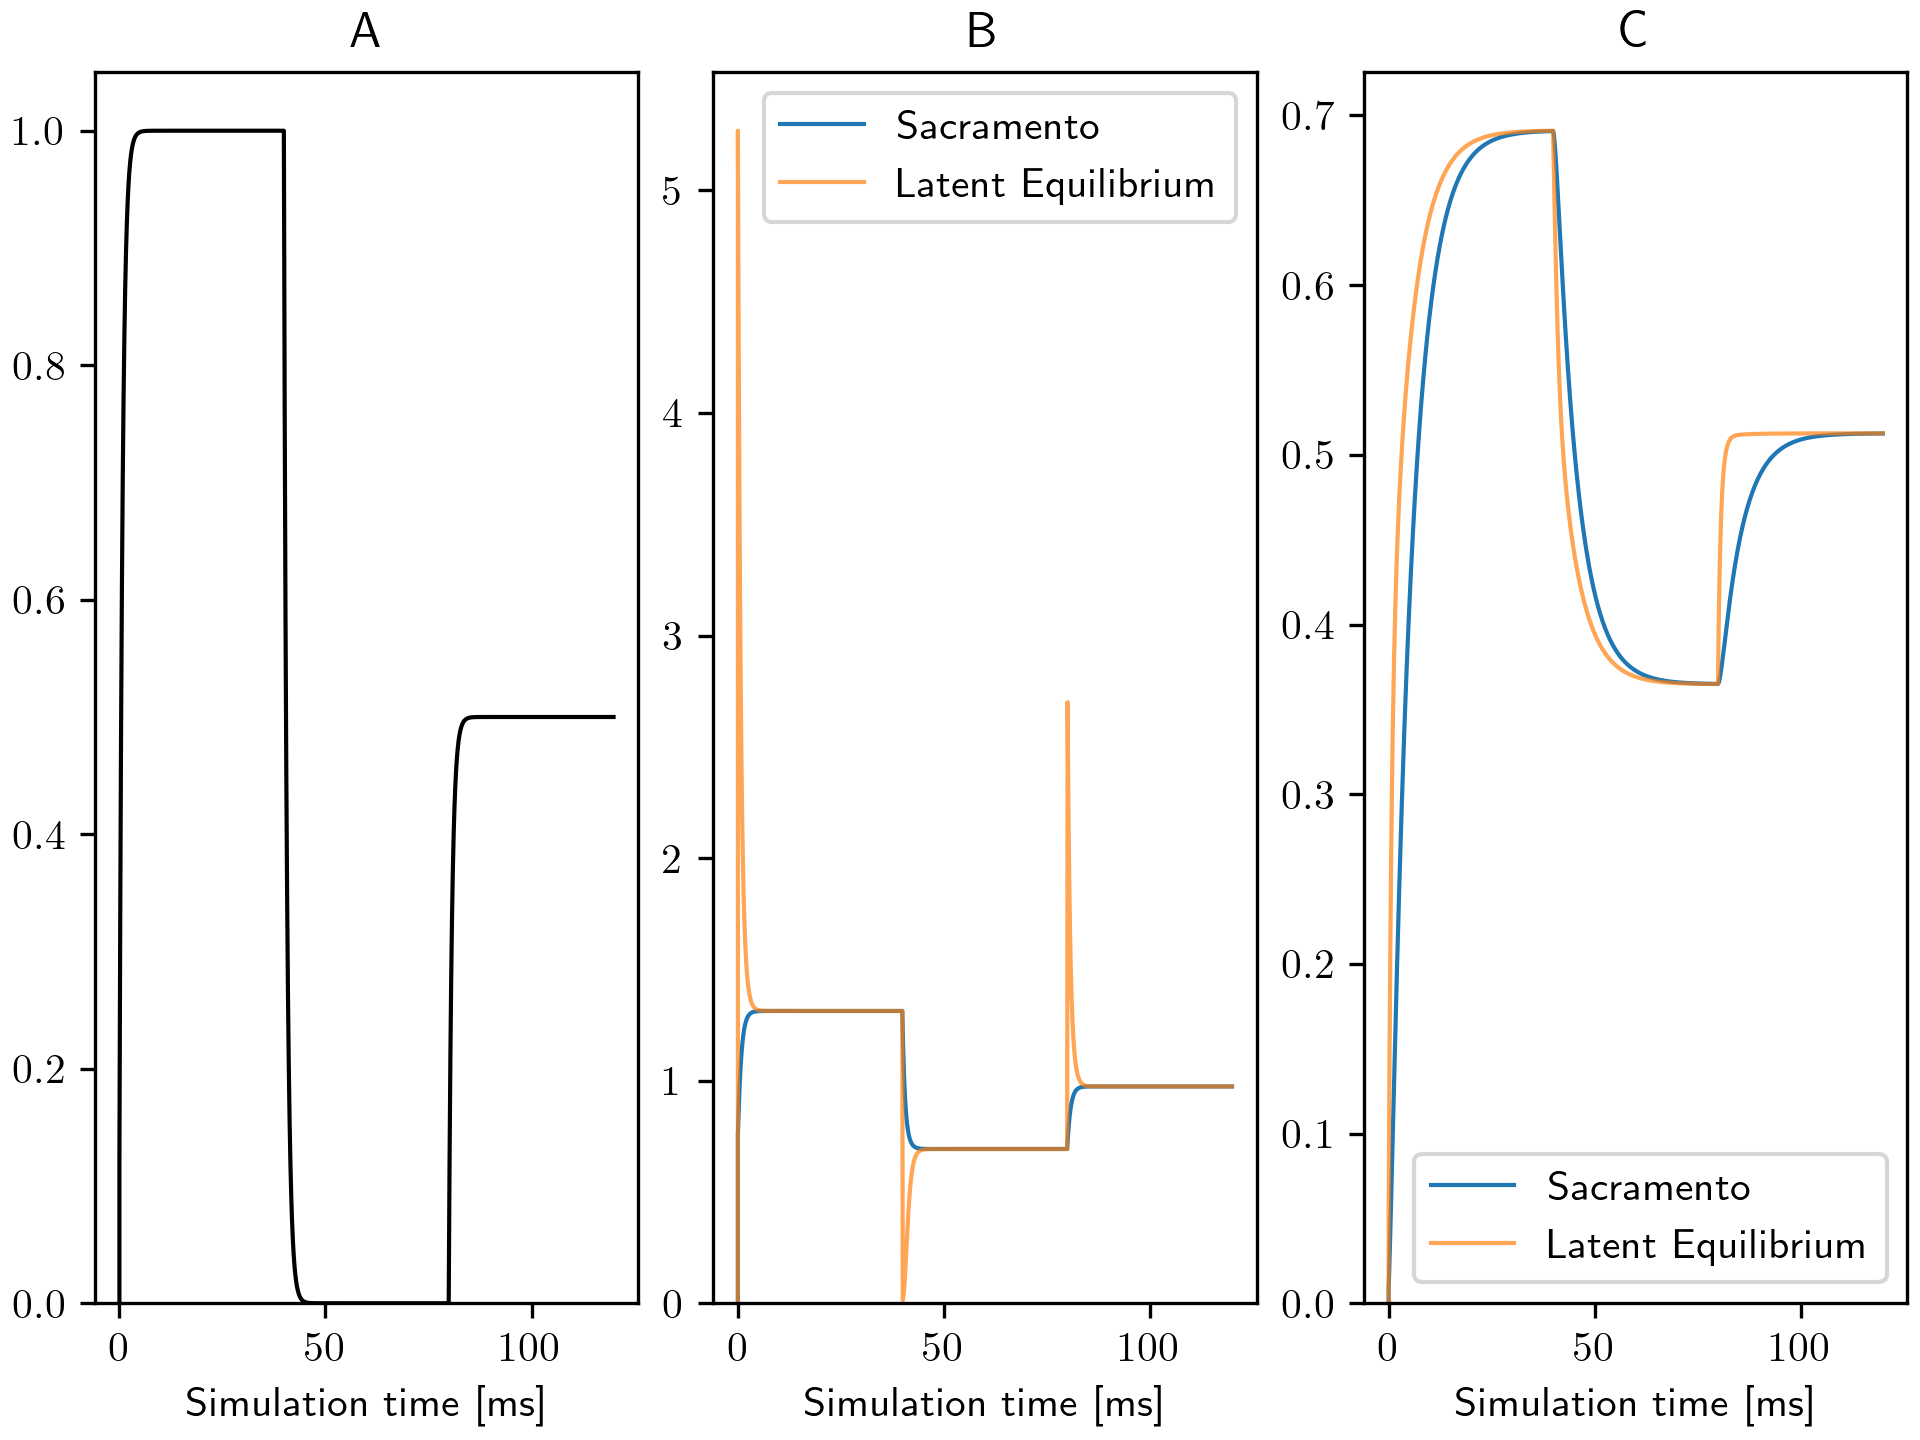
\includegraphics[width=0.9\textwidth]{fig_le_comparison}
  \caption{Comparison of signal transmission between Sacramento model and a neuron using Latent Equilibrium. \textbf{A:}
    Somatic voltage of a single input neuron. Three different currents are injected for $40ms$ each. The input neuron
    $x$ acts as a low pass filter on these currents with time constant $\tau_x = 0.8 ms$. \textbf{B:} Activation of the
    input neuron using Sacramento dynamics $\phi(u_x)$ (blue), and Latent equilibrium $\phi(\breve{u}_x)$ (orange). Note
    how strongly the LE neuron reacts to changes in somatic voltage, leading to spikes in activation. After the input
    neuron has reached its steady-state ($\dot{u}_x = 0$), both types evoke the same activation. \textbf{C:} Somatic
    potential of a simplified pyramidal neuron responding to signals sent from the input neuron (color scheme as in B).
    When a presynaptic neuron employs LE dynamics, postsynaptic voltage responds more quickly to changes in the input,
    leading to a faster convergence on a steady state.}
  \label{fig-comparison-le}
\end{figure}


\begin{figure}
  \centering
  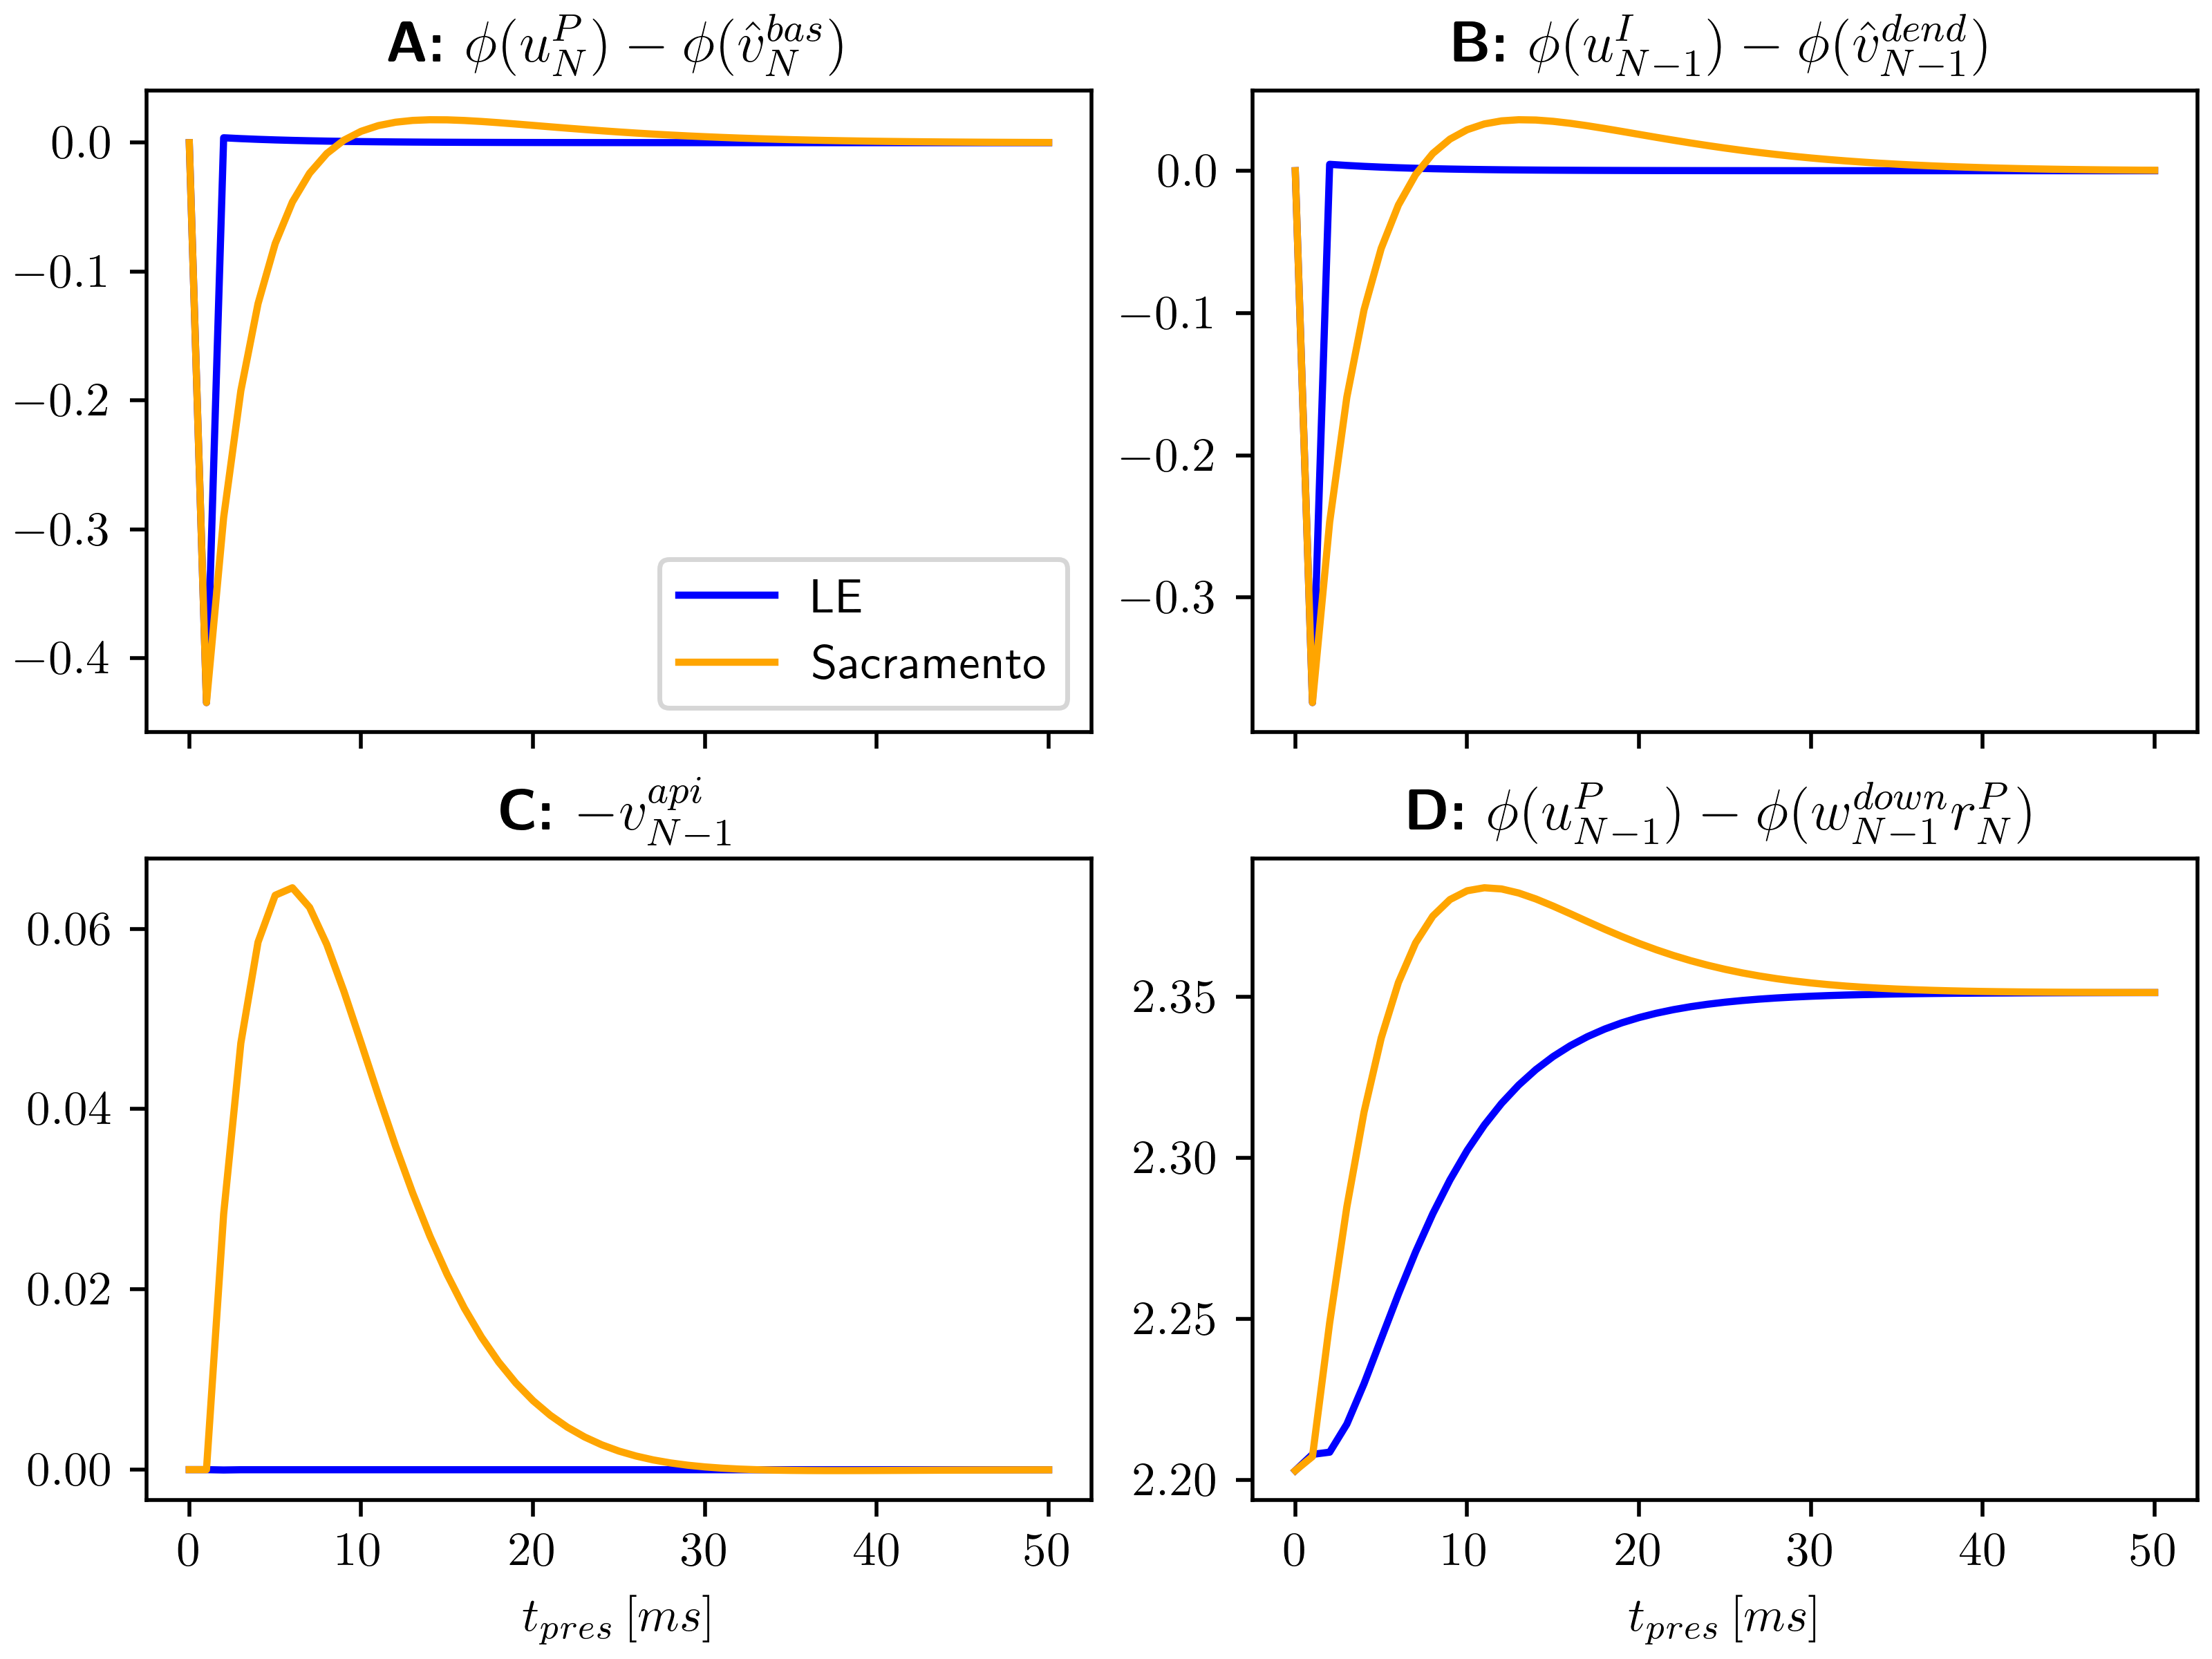
\includegraphics[width=0.9\textwidth]{fig_2_le_dendritic_errors}
  \caption{Comparison of stimulus presentation effects on the local error terms from Equations
    \ref{eq-delta_w_up}-\ref{eq-delta_w_down}. Depicted are error terms for individual neurons of a network with one
    hidden layer ($N=3$) that was fully trained on the Bars dataset \todo{ref}. When employing Sacramento dynamics
    (orange), dendritic errors exhibit longer and more intense deviations, while errors in an identical LE network
    (blue) are cancelled out much sooner. \textbf{A:} Basal dendritic error for a pyramidal neuron at the output layer.
    \textbf{B:} Dendritic error for a hidden layer Interneuron. \textbf{C:} Proximal apical error for a hidden layer
    Pyramidal neuron. For this case the difference between the two networks is most striking, as errors for the LE
    network exhibit almost no deviation from rest. \textbf{D:} Distal apical error for the same pyramidal neuron. Note
    that this error term does not converge to zero for either network even after training is complete, which will be
    discussed \todo{later}.}
  \label{fig-error-comp-le}
\end{figure}

In addition to using the prospective \todo{introduce term} somatic potential for the neuronal transfer function, it is
also used in the plasticity rule. The Urbanczik-Senn plasticity is therefore updated to compute dendritic error from the
prospective somatic potential $\dot{w}_{ij}= \eta \ ( \phi(\breve{u}_i^{som}) - \phi(\hat{v}_i^{bas}) ) \
  \phi(\breve{u}_j^{som})^T$. Much like for the transfer function, this change serves to increase the responsiveness of
the network to input changes. \newline


\todo{keep the following section?}
Besides the using a prediction of future somatic activity for neuronal transfer and plasticity, \cite{Haider2021}
further alter the plasticity rule by means of their implementation. While the simulations by
\cite{sacramento2018dendritic} strictly conforms to the equations above, the new implementation
(\href{https://github.com/neurips}{GitHub}) . The fundamental building block of a network here is a layer, which is
represented in code as an instance of the class \texttt{Layer}. Each instances holds information about its corresponding
pyramidal- and interneurons. It also holds information about the synaptic connections between the two populations, as
well as all incoming feedforward and feedback pyramidal synapses. A layer has two class methods that are fundamental to
its computation; \texttt{update()} computes membrane potential derivatives and synaptic weight changes given pyramidal
neuron activations from the previous and subsequent layers. \texttt{apply()} updates weights and membrane potentials
from the previously calculated changes. Layers are processed in order from input to output layer, where all of them
receive the \texttt{update()} signal first, before \texttt{apply()} is called on all of them. This ordering ensures,
that changes in activation do not cascade through the layers and lead to excessive activations at the output. Yet, since
next layer activations at time $t$ have not been computed, top down information is always delayed by one timestep.
\todo{evaluate importance of this}


Thus, the equations for membrane updates change slightly:

\begin{align}
  \dot{W_{ij}}(t)    & = \eta (\phi(u_i) - \phi(\alpha v^{basal}_i(t))) \phi(u_j)                             \\
  \Delta W_{ij}(t,T) & = \int_t^T dt' \ \eta \  (\phi(u_i^{t'}) - \phi(\widehat{v_i^{t'}})) \  \phi(u_j^{t'}) \\
  \Delta W_{ij}(t,T) & = \eta \int_t^T dt' \  (\phi(u_i^{t'}) - \phi(\widehat{v_i^{t'}})) \ \phi(u_j^{t'})    \\
  V_i^*              & = \phi(u_i^{t'}) - \phi(\widehat{v_i^{t'}})                                            \\
  s_j^*              & = \kappa_s * s_j
\end{align}



\begin{align}
  \phi(V^{som}) & \rightarrow \phi(\breve{V}^{som}) \\
  \breve{V}     & := V + \tau^m \dot{V}             \\
\end{align}
\begin{align}
  \frac{d}{dt} W_{ba} & = \eta (\phi(V_b^{som}) - \phi(\alpha V_b^{dend})) \phi(V_a^{som})                         \\
  \frac{d}{dt} W_{ba} & = \eta (\phi(\breve{V}_b^{som}) - \phi(\alpha \breve{V}_b^{dend})) \phi(\breve{V}_a^{som})
\end{align}


\section{rate neurons in NEST}

\section{simulation details/updates}

All voltages need to be reset between simulations!

\begin{itemize}
  \item injections into the network
  \item output layer readout
  \item interoperability of networks
  \item

\end{itemize}

